% +------------------------------------------------------------------------+
% | Reference manual page: Subdivision_surfaces_3.tex
% +------------------------------------------------------------------------+
% | 03/01/2005   Le-Jeng Andy Shiue
% | Package: Subdivision_surface_3
% | 
\RCSdef{\RCSSubdivisionRev}{$Revision$}
\RCSdefDate{\RCSSubdivisionDate}{$Date$}
% +------------------------------------------------------------------------+

\ccRefPageBegin

%%RefPage: end of header, begin of main body
% +------------------------------------------------------------------------+


\begin{ccRefClass}{Subdivision_surfaces_3}

\ccDefinition

Subdivision surfaces of an input polyhedral mesh
are generated by recursive topology refinement and geometry
smoothing. \ccClassTemplateName\ consists a set of static 
template functions (i.e.~refinement hosts) corresponding 
to four refinement schemes practically used by subdivision surfaces. 
Each refinement host, parameterized with a geometry policy,
%consisting of a set of geometry stencils, 
refines the input mesh, maintains the stencils, and smooths the 
refined mesh by the geometry policy.

A set of subdivision functions are also provided  
for Catmull-Clark, Loop, Doo-Sabin and $\sqrt{3}$ subdivision.
These subdivision functions are pre-parameterized with the
subdivision policies.

%% \begin{ccTexOnly}
%%     \vspace{-7mm}
%%     \begin{center}
%%       \parbox{0.4\textwidth}{%
%%         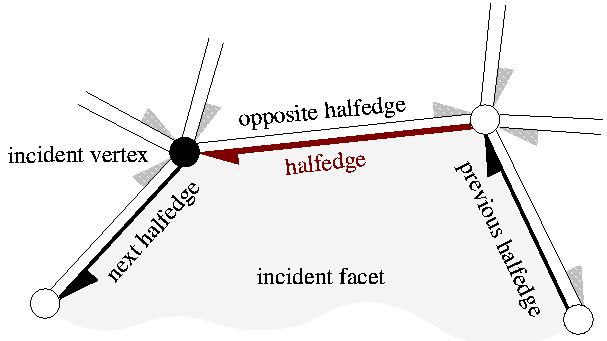
\includegraphics[width=0.4\textwidth]{Polyhedron_ref/fig/halfedge}%
%%       }
%%     \end{center}
%%     \vspace{-5mm}
%% \end{ccTexOnly}

%% \begin{ccHtmlOnly}
%%     <CENTER>
%%     <A HREF="fig/halfedge.gif">
%%         <img src="fig/halfedge_small.gif" alt="Halfedge Diagram"></A><P>
%%     </CENTER>
%% \end{ccHtmlOnly}

\ccInclude{CGAL/Subdivision_surfaces_3.h}

\ccParameters

The full template declaration of \ccClassTemplateName\ states one
template parameters:

\begin{tabbing}
\ccc{template <} \=\ccc{class  _Poly>} \ccc{class Subdivision_surfaces_3;}
\end{tabbing}
   
The \ccc{_Poly} parameter requires a model of 
the \ccc{Polyhedron_3} concept as argument. The storage structure
of \ccc{_Poly} is required to be a FIFO structure (e.g.~vector or list).
Refined vertices are generated in a specific order that
is used to maintain the stencils, hence no explicit flag is required
to maintain the stencils. To support the geometry smoothing, \ccc{_Poly}
is required to define \ccc{Point_3} as the position holder.

%% \ccTypes

%% \ccNestedType{Traits}{traits class selected for \ccc{PolyhedronTraits_3}.}
%% \ccGlue
%% \ccNestedType{Items}{items class selected for \ccc{PolyhedronItems_3}.}
%% \ccGlue



%% % +-----------------------------------+
%% \begin{ccAdvanced}
%% \ccHeading{Types for Tagging Optional Features}

%% \ccNestedType{Supports_facet_plane}{\ccc{Facet::plane()}.}
%% \ccGlue
%% \ccNestedType{Supports_removal}{supports removal of individual elements.}

%% \end{ccAdvanced}

\ccCreation
%\ccCreationVariable{P}

\ccClassTemplateName\ serves as a template namespace, hence no constructor
is defined. 

%and provides a 
%set of static functions of refinements. 

%No object of \ccClassTemplateName\ is reuqired to be 
%instantiated before calling subdivision or generic refinement functions.

% +-----------------------------------+
\ccHeading{Refinement hosts}

\ccThree{}{}{}
\ccMethod{template <template <typename> class _S> 
void PQQ(Polyhedron& p, _S<Polyhedron> rule, int step)}
{refine the mesh \ccc{p} with the PQQ refinement
\ccc{step} times, and smooth the refined \ccc{p} with the geometry 
masks \ccc{rule}.}
%% \begin{ccTexOnly}
%%     \begin{center}
%%       \parbox{0.636\textwidth}{%
%%           \includegraphics[width=0.636\textwidth]%
%%               {Polyhedron_ref/fig/euler_loop}%
%%       }
%%     \end{center}
%% \end{ccTexOnly}
%% \begin{ccHtmlOnly}
%%     <CENTER>
%%     <img src="fig/euler_loop.gif" alt="Euler Operator: Loop"><P>
%%     </CENTER>
%% \end{ccHtmlOnly}

\ccMethod{template <template <typename> class _S> 
void PTQ(Polyhedron& p, _S<Polyhedron> rule, int step)}
{refine the mesh \ccc{p} with the PTQ refinement 
\ccc{step} times, and smooth the refined \ccc{p} with the geometry 
masks \ccc{rule}.}

\ccMethod{template <template <typename> class _S> 
void DQQ(Polyhedron& p, _S<Polyhedron> rule, int step)}
{refine the mesh \ccc{p} with the DQQ refinement 
\ccc{step} times, and smooth the refined \ccc{p} with the geometry 
masks \ccc{rule}.}

\ccMethod{template <template <typename> class _S> 
void Sqrt3(Polyhedron& p, _S<Polyhedron> rule, int step)}
{refine the mesh \ccc{p} with the $\sqrt{3}$ triangulation 
\ccc{step} times, and smooth the refined \ccc{p} with the geometry 
masks \ccc{rule}.}


% +-----------------------------------+
\ccHeading{Subdivision Surfaces}
\ccThree{}{}{}

\ccMethod{void CatmullClark_subdivision(Polyhedron& p, int step)}
{apply Catmull-Clark subdivision \ccc{step} times on the mesh \ccc{p}.}

\ccMethod{void Loop_subdivision(Polyhedron& p, int step)}
{apply Loop subdivision \ccc{step} times on the mesh \ccc{p}. 
The mesh \ccc{p} can only consist of triangle facets.}

\ccMethod{void DooSabin_subdivision(Polyhedron& p, int step)}
{apply Doo-Sabin subdivision \ccc{step} times on the mesh \ccc{p}.}

\ccMethod{void Sqrt3_subdivision(Polyhedron& p, int step)}
{apply $\sqrt{3}$ subdivision \ccc{step} times on the mesh \ccc{p}.
The mesh \ccc{p} can only consist of triangle facets.}

\ccExample

This example program applies the Catmull-Clark subdivision on a
read-in polyhedral mesh.

\ccIncludeExampleCode{Subdivision_surfaces_3/CatmullClark_subdivision.C}

\ccSeeAlso

\ccRefIdfierPage{CGAL::PQQ_stencil}\\
\ccRefIdfierPage{CGAL::DQQ_stencil}\\
\ccRefIdfierPage{CGAL::Linear_stencil}\\
\ccRefIdfierPage{CGAL::CatmullClark_stencil}\\
\ccRefIdfierPage{CGAL::Loop_stencil}\\
\ccRefIdfierPage{CGAL::Sqrt3_stencil}\\

\end{ccRefClass}

% +------------------------------------------------------------------------+
%%RefPage: end of main body, begin of footer
\ccRefPageEnd
% EOF
% +------------------------------------------------------------------------+
